
\section{Introduction}

In recent years, large-scale learned models such as 

\begin{figure}[t]
    \centering
    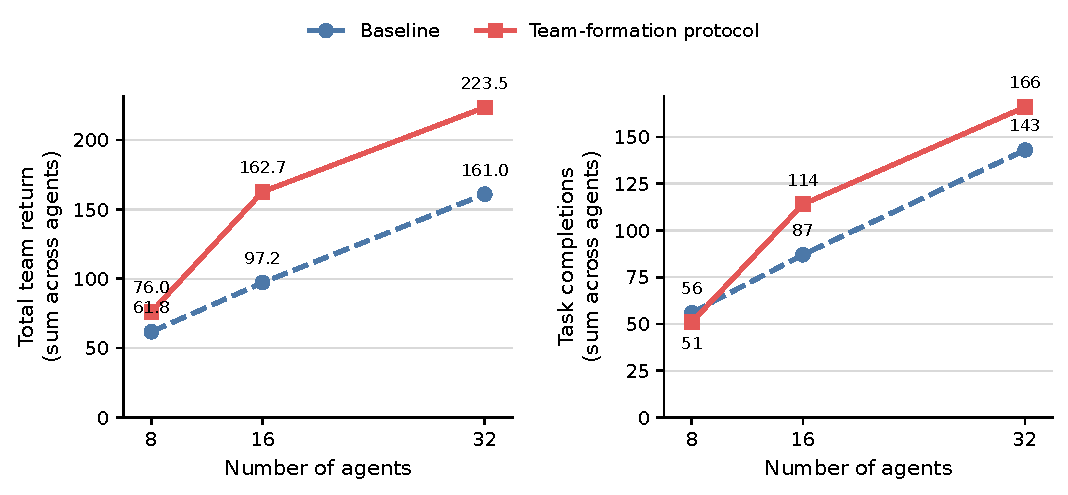
\includegraphics[width=\linewidth]{Figures/20260721_absolute_team_performance.pdf}
    \caption{...}
    \label{fig:absolute-team-performance}
\end{figure}

\section{Related Works}

\subsection{Market-Based Coordination}

\subsubsection{Contract Net Market}

\subsubsection{CU Credits}

\subsection{Context Management for Instruction Adherence}

\subsection{Alem Environment}

\section{Methods}

We will conduct a series of experiments to verify the effectiveness of dynamic teaming within Alem.

\textit{Key change we need to make: As teams scale, we need to ensure teams required for tasks don't go above 4, as some tasks requre all agents to interact with an object, so we choose max 3 agents per task for our experiments.}

1- Collect baseline results for 1,2,3,6 agent populations (3 seeds each)
2- examine methods of constructing teams using decentralized methods
3- evaluate the complexity 



\subsection{Empirical Results}

We evaluated the unchanged Source condition across $N \in \{1,2,3,4,6\}$ with three seeded episodes per population. The results were non-monotonic. Mean Total score increased from 3.379 for the single-agent condition to 9.752 at $N=3$ and 9.574 at $N=4$, before declining to 6.738 at $N=6$. The gains at intermediate populations came mainly from coordination-related achievement, while the six-agent setting showed lower task diversity and higher execution cost.

For the coordination mechanism, we tested Open Volunteer. It completed 12 synthetic six-agent cells, formed 15/15 true-feasible teams, matched the exact whole allocation in 10/12 cells and the exact task rosters in 12/15, and kept mean utility regret low at 0.00566. It also hit full reward and oracle-allocation coverage in all 12 cells with no transport errors, incomplete responses, or truncation across 293 calls, and a mean raw-cost delta of $+4.9167$. 

\begin{table}[t]
\centering
\small
\resizebox{\textwidth}{!}{%
\begin{tabular}{@{}rrrrrrrrrrr@{}}
\toprule
Agents & Episodes & Base \% & Coord. \% & Total \% & Return & Team-unique unlocks & Summed agent unlocks & Actual ticks & Actionable turns & Tick time \\
\midrule
1 & 3 & 3.379 & -- & 3.379 & 7.133 & 7.33 & 7.33 & 200.0 & 100.0\% & 4.55s \\
2 & 3 & 5.376 & 3.774 & 4.699 & 14.283 & 10.33 & 16.00 & 200.0 & 95.8\% & 6.90s \\
3 & 3 & 12.596 & 5.870 & 9.752 & 21.678 & 19.33 & 36.33 & 197.0 & 86.9\% & 8.66s \\
4 & 3 & 8.602 & 10.901 & 9.574 & 20.375 & 19.33 & 42.33 & 200.0 & 94.1\% & 10.33s \\
6 & 3 & 8.141 & 4.822 & 6.738 & 11.883 & 15.00 & 42.33 & 200.0 & 90.1\% & 14.65s \\
\bottomrule
\end{tabular}}
\caption{Population means for the completed Source population screen. Base, Coordination, and Total are reward-weighted paper scores on a 0--100 scale. Coordination is undefined for the single-agent condition.}
\label{tab:population-means}
\end{table}





\section{Conclusion \& Future Work}

\section{Limitations}